% ============================================================
%  Radar Sinyal Sınıflandırma ve Gürültü Giderme — Beamer Sunumu
%  Overleaf'te pdfLaTeX ile derleyin.
%  Sonuç görselleri ../results/ klasöründen alınır; bu klasörü
%  Overleaf projesine yüklemeyi unutmayın (veya \graphicspath'i güncelleyin).
% ============================================================
\documentclass[aspectratio=169]{beamer}

\usepackage[T1]{fontenc}
\usepackage[utf8]{inputenc}    % Türkçe karakterler (ç ğ ı İ ş ö ü)
\usepackage{lmodern}
\usepackage{graphicx}
\usepackage{booktabs}
\usepackage{amssymb}
\usepackage{tikz}
\usetikzlibrary{arrows.meta, positioning}

\usetheme{Madrid}
\usecolortheme{whale}
\setbeamertemplate{navigation symbols}{}
\setbeamertemplate{caption}{\raggedright\insertcaption\par}
\setbeamerfont{block title}{size=\small}

\graphicspath{{../results/}}

% ---- Renkler (pipeline kutuları) ----
\definecolor{cData}{RGB}{52,152,219}
\definecolor{cDeno}{RGB}{46,204,113}
\definecolor{cClf}{RGB}{155,89,182}
\definecolor{cEdge}{RGB}{230,126,34}

\title[Radar Sinyal Sınıflandırma]{Gürültü Giderme Tabanlı\\ Çok Etiketli Radar Sinyal Sınıflandırma}
\subtitle{Spektrogram Denoising $+$ Sınıflandırma $+$ Parametre Çıkarımı}
\author{}
\institute{}
\date{}

\begin{document}

% ---------------------------------------------------------
\begin{frame}[plain]
  \titlepage
\end{frame}

% ---------------------------------------------------------
\begin{frame}{İçerik}
  \tableofcontents
\end{frame}

% =========================================================
\section{Motivasyon}
% =========================================================
\begin{frame}{Problem ve Motivasyon}
  \begin{block}{Neden zor?}
    \begin{itemize}
      \item Elektronik harp / ESM alıcıları, yoğun bir elektromanyetik ortamda
            \textbf{çok sayıda radar sinyalini aynı anda} görür.
      \item Düşük SNR'da sinyaller spektrogramda \textbf{gürültüye gömülür};
            klasik eşikleme ve el yapımı öznitelikler yetersiz kalır.
      \item Aynı zaman-frekans penceresinde \textbf{birden fazla modülasyon türü}
            üst üste binebilir (çok etiketli problem).
    \end{itemize}
  \end{block}
  \begin{block}{Yaklaşımımız}
    Önce \textbf{öğren-tabanlı gürültü giderme}, ardından \textbf{çok etiketli
    sınıflandırma}, son olarak \textbf{parametre (PRI/PW/BW/Fc) çıkarımı}.
  \end{block}
\end{frame}

\begin{frame}{Katkılar}
  \begin{enumerate}
    \item Gürültülü ve temiz spektrogram \textbf{çiftlerini} otomatik üreten,
          çok çerçeveli, çok etiketli bir \textbf{sentetik veri seti} üreteci.
    \item Spektrogramı temizleyen \textbf{ResNet-18 + U-Net} tabanlı bir denoiser.
    \item Gürültülü ve gürültüsü giderilmiş girişleri \textbf{karşılaştıran}
          çok etiketli \textbf{GoogLeNet} sınıflandırıcı.
    \item Temizlenmiş spektrogramdan \textbf{Radar Tanımlayıcı Kelime (RDW)}
          çıkaran kenar/kümeleme boru hattı.
  \end{enumerate}
  \vfill
  \begin{center}\small
  Sınıflar: \textbf{LFM, NLFM, FSK, Barker, Frank, P\_All, none} (7 sınıf)
  \end{center}
\end{frame}

% =========================================================
\section{Genel Mimari}
% =========================================================
\begin{frame}{Uçtan Uca Boru Hattı}
  \centering
  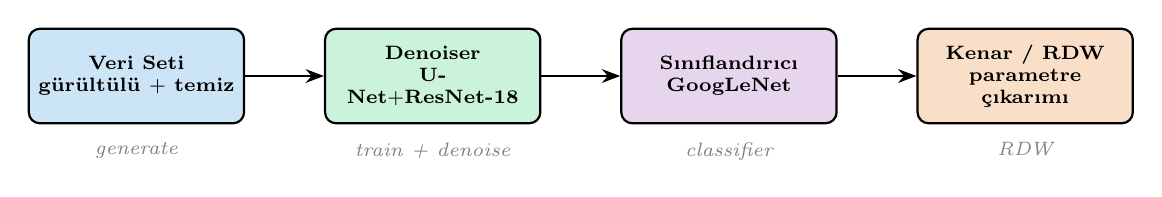
\begin{tikzpicture}[
      node distance=7mm and 10mm,
      box/.style={rounded corners, draw, thick, text width=2.5cm,
                  align=center, minimum height=1.2cm, font=\scriptsize\bfseries},
      lbl/.style={font=\scriptsize\itshape, text=gray},
      >={Stealth[]}, thick]
    \node[box, fill=cData!25]  (data) {Veri Seti\\ \scriptsize gürültülü $+$ temiz};
    \node[box, fill=cDeno!25, right=of data] (deno) {Denoiser\\ \scriptsize U-Net$+$ResNet-18};
    \node[box, fill=cClf!25,  right=of deno] (clf)  {Sınıflandırıcı\\ \scriptsize GoogLeNet};
    \node[box, fill=cEdge!25, right=of clf]  (edge) {Kenar / RDW\\ \scriptsize parametre çıkarımı};
    \draw[->] (data) -- (deno);
    \draw[->] (deno) -- (clf);
    \draw[->] (clf)  -- (edge);
    \node[lbl, below=1mm of data] {generate};
    \node[lbl, below=1mm of deno] {train + denoise};
    \node[lbl, below=1mm of clf]  {classifier};
    \node[lbl, below=1mm of edge] {RDW};
  \end{tikzpicture}
  \vfill
  \begin{itemize}\small
    \item Her aşama \textbf{bağımsız bir MATLAB modülü}dür; ayrı çalıştırılabilir.
    \item Denoiser ve sınıflandırıcı, \textbf{224$\times$224} gri spektrogram
          yamaları üzerinde çalışır.
  \end{itemize}
\end{frame}

\begin{frame}{Radar Sinyal Türleri}
  \centering
  \renewcommand{\arraystretch}{1.2}
  \begin{tabular}{@{}ll@{}}
    \toprule
    \textbf{Tür} & \textbf{Açıklama} \\
    \midrule
    LFM     & Doğrusal frekans modülasyonu (chirp) \\
    NLFM    & Doğrusal olmayan FM (düşük yan lob) \\
    FSK     & Frekans kaydırmalı anahtarlama \\
    Barker  & Barker bifaz kodu (7, 11, 13) \\
    Frank   & Frank polifaz kodu ($N=4,8,16$) \\
    P\_All  & P1--P4 polifaz kodları \\
    none    & Sinyal yok (yalnızca gürültü) \\
    \bottomrule
  \end{tabular}
  \vfill
  {\small Her yama \textbf{aynı anda birden fazla} türü içerebilir
  (en fazla 3) $\Rightarrow$ çok etiketli sınıflandırma.}
\end{frame}

% =========================================================
\section{Veri Seti}
% =========================================================
\begin{frame}{Veri Seti Üretimi}
  \begin{columns}[T]
    \begin{column}{0.54\textwidth}
      \textbf{Sahne simülasyonu}
      \begin{itemize}\small
        \item 10 kısa çerçeveden oluşan \textbf{IQ sahne} ($f_s = 30$ MHz).
        \item Rastgele tür, taşıyıcı $F_c$, PW, PRI, BW; guard-band ile $F_c$ ayrımı.
        \item 4 SNR seviyesi karıştırılır: $\{20, 10, 0, -10\}$ dB.
      \end{itemize}
      \textbf{Spektrogram}
      \begin{itemize}\small
        \item STFT: 256 nokta, Hamming, \%75 örtüşme, ortalanmış.
        \item dB $\rightarrow$ \textbf{sabit global ölçek} ile $[0,1]$'e eşlenir.
      \end{itemize}
      \textbf{Yama çıkarımı}
      \begin{itemize}\small
        \item Uzun spektrogram ($224\times2240$) $\rightarrow$ \%50 örtüşen
              $224\times224$ yamalar (hop $=112$).
        \item Boş (none) yamalar seyreltilir (denge için).
      \end{itemize}
    \end{column}
    \begin{column}{0.46\textwidth}
      \centering
      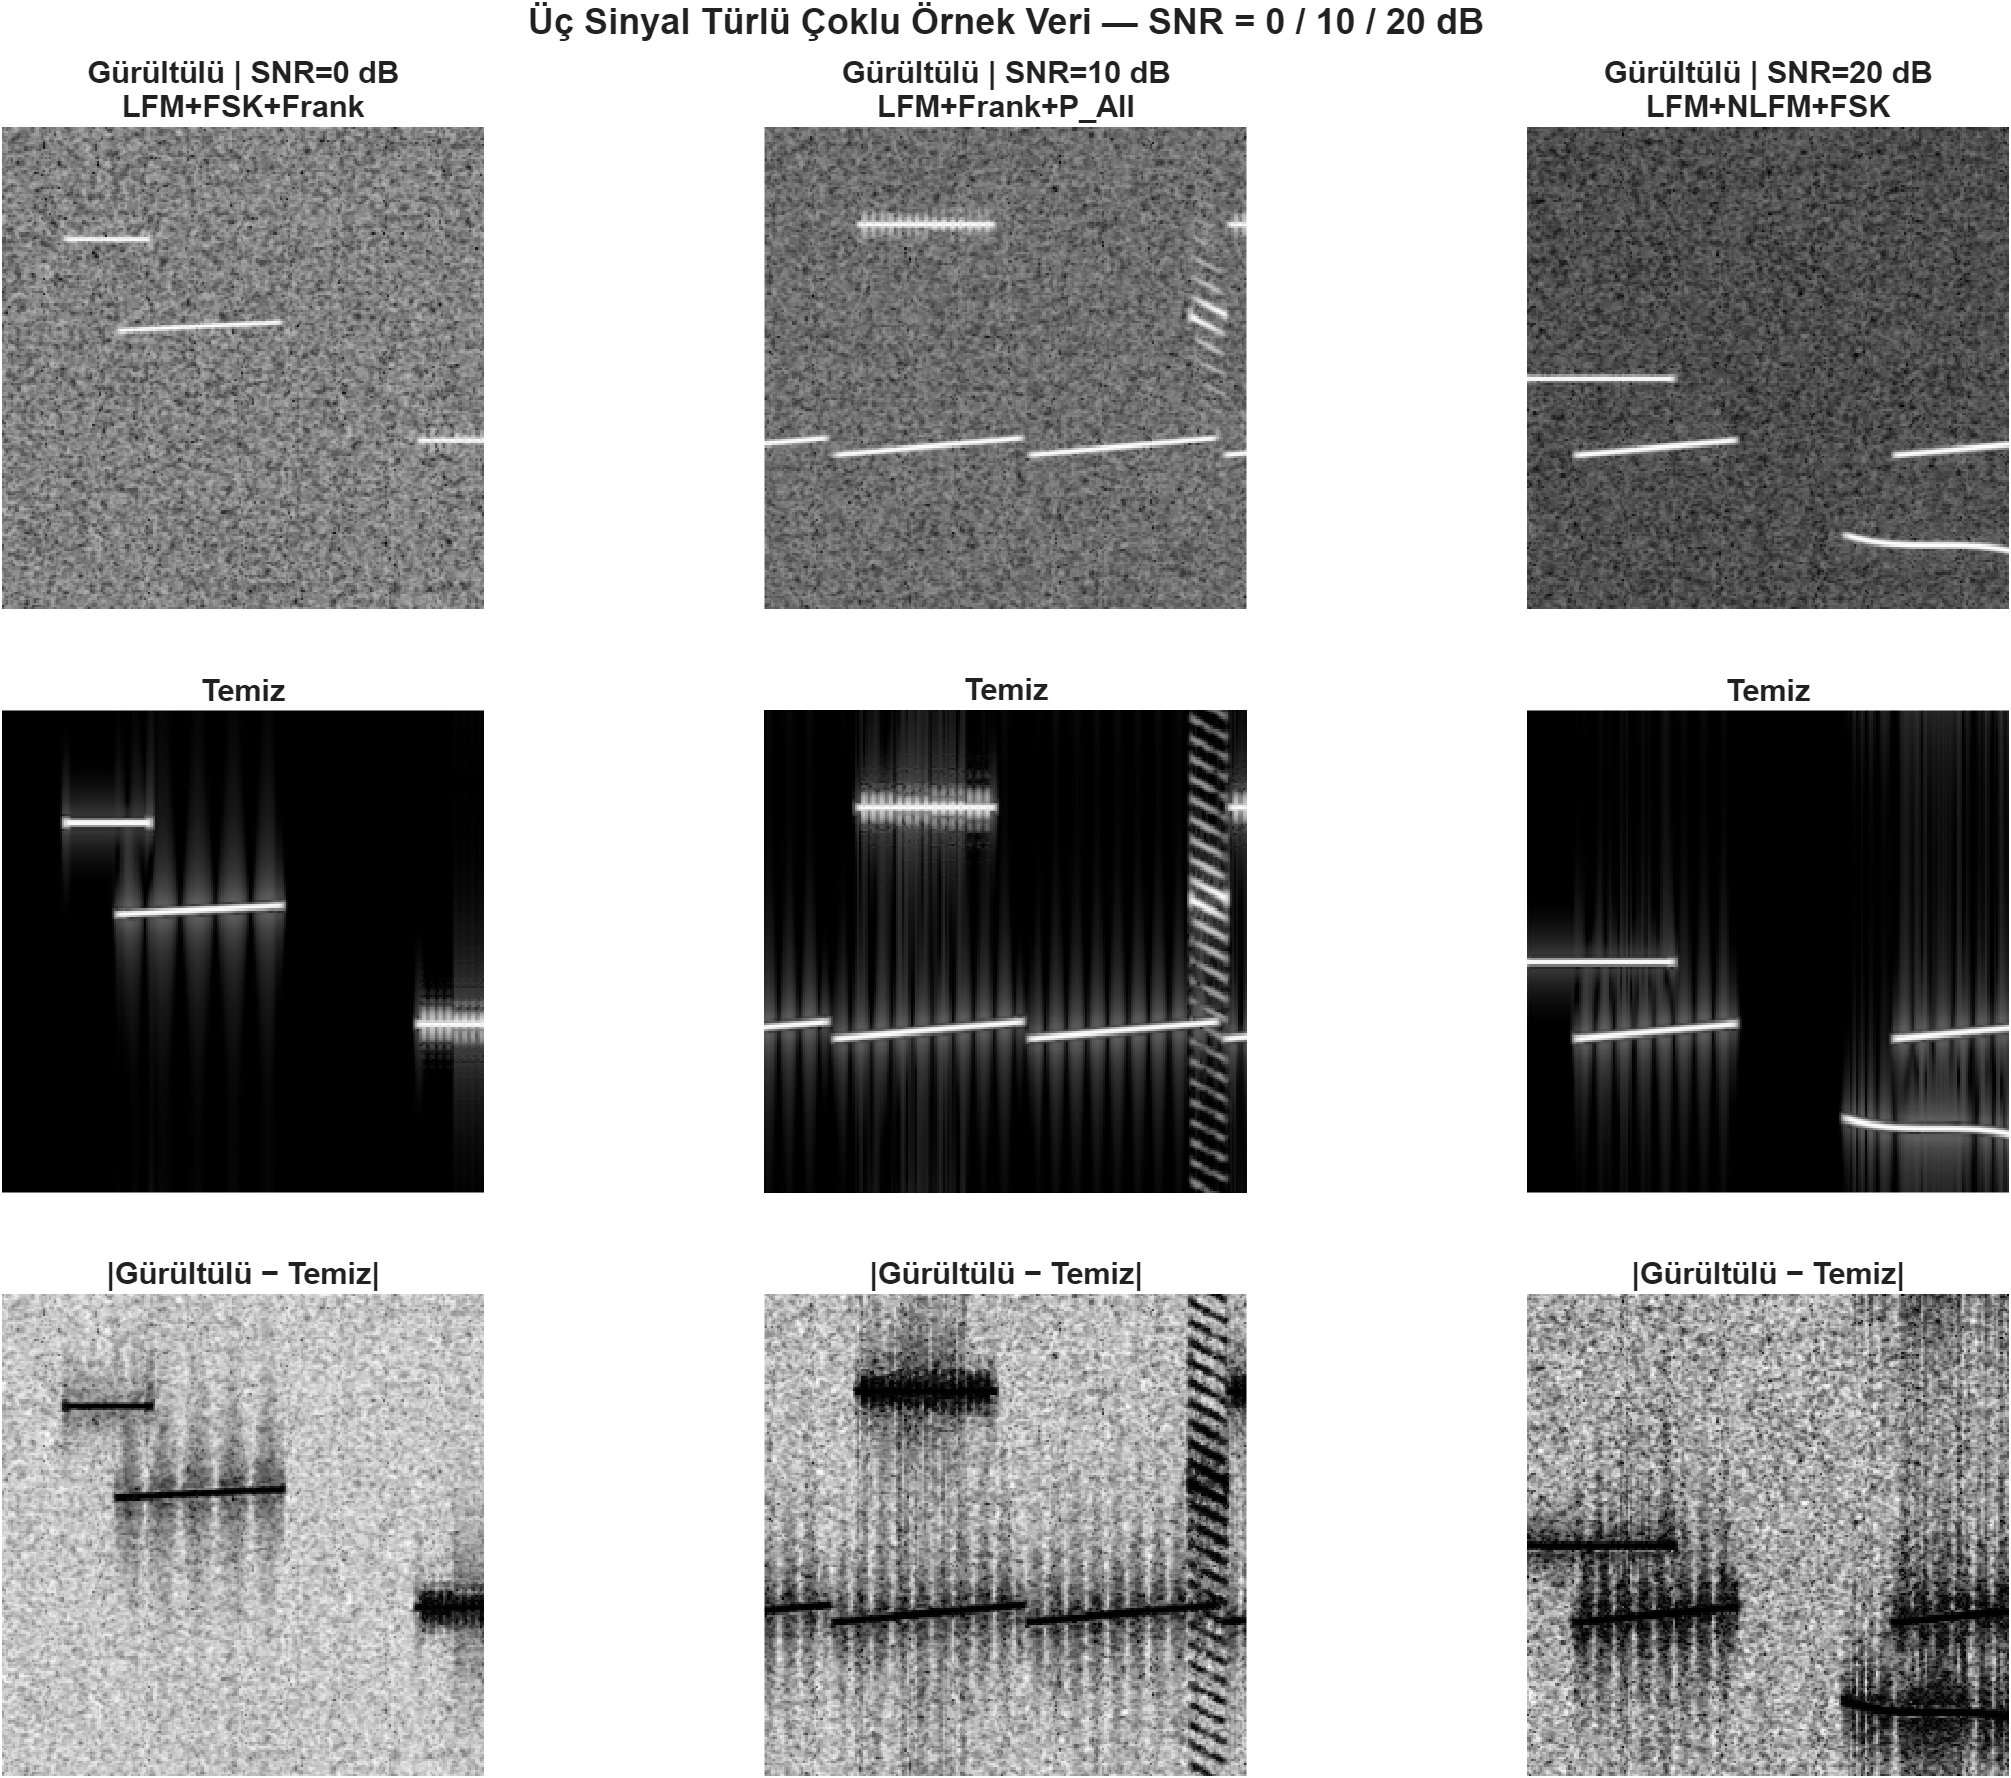
\includegraphics[width=\linewidth]{example_3x3_SNR_0_10_20_numTypes3.png}\\[2pt]
      {\scriptsize Üstten alta: \textbf{gürültülü} / \textbf{temiz} /
       \textbf{fark}; soldan sağa SNR $=0/10/20$ dB.}
    \end{column}
  \end{columns}
\end{frame}

\begin{frame}{Her Yama İçin Ne Kaydediliyor?}
  \begin{itemize}
    \item \texttt{specNoisyGray/} — gürültülü gri spektrogram (denoiser girişi,
          sınıflandırıcı-1 girişi).
    \item \texttt{specCleanGray/} — temiz referans (denoiser hedefi, PSNR/SSIM referansı).
    \item \texttt{specDenoisedGray/} — denoiser çıktısı (sınıflandırıcı-2 girişi).
    \item \texttt{meta/*.json} — sahne meta verisi (SNR, tür, $F_c$, PRI \dots).
    \item \texttt{labels.csv} — her yama için \textbf{7 sınıflık ikili etiket} vektörü.
  \end{itemize}
  \vfill
  \begin{center}\small
    Böylece hem \textbf{denoising} (çift: gürültülü$\rightarrow$temiz) hem de
    \textbf{sınıflandırma} (yama$\rightarrow$etiket) tek veri setinden beslenir.
  \end{center}
\end{frame}

% =========================================================
\section{Gürültü Giderme}
% =========================================================
\begin{frame}{Denoiser Mimarisi}
  \begin{columns}[T]
    \begin{column}{0.55\textwidth}
      \begin{itemize}\small
        \item \textbf{Enkoder:} ImageNet ön-eğitimli \textbf{ResNet-18}
              (sınıflandırma başlığı kaldırılmış).
        \item \textbf{Dekoder:} \textbf{U-Net} tarzı; transposed-conv ile 5 kademeli
              yukarı örnekleme.
        \item \textbf{Skip bağlantıları:} enkoderin ara katmanları dekodere
              eklenir $\Rightarrow$ ince yapı korunur.
        \item Giriş $224\times224\times3$ (gri, 3 kanala kopyalanır),
              çıkış $224\times224\times1$ \textbf{regresyon}.
      \end{itemize}
      \begin{block}{Eğitim}\scriptsize
        Kayıp: MSE \;|\; Adam, $\text{lr}=10^{-4}$ \;|\; batch $=8$ \;|\;
        40 epoch \;|\; ince ayar (LR faktörü $0.2$) \;|\; checkpoint $+$ en iyi model.
      \end{block}
    \end{column}
    \begin{column}{0.45\textwidth}
      \centering
      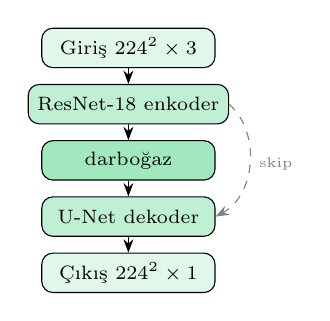
\begin{tikzpicture}[
          n/.style={draw, rounded corners, minimum width=2.2cm, minimum height=5mm,
                    font=\scriptsize, align=center},
          >={Stealth[]}]
        \node[n, fill=cDeno!15] (i)  {Giriş $224^2\times3$};
        \node[n, fill=cDeno!30, below=2mm of i] (e1) {ResNet-18 enkoder};
        \node[n, fill=cDeno!45, below=2mm of e1] (b)  {darboğaz};
        \node[n, fill=cDeno!30, below=2mm of b] (d1) {U-Net dekoder};
        \node[n, fill=cDeno!15, below=2mm of d1] (o)  {Çıkış $224^2\times1$};
        \draw[->] (i)--(e1); \draw[->] (e1)--(b);
        \draw[->] (b)--(d1); \draw[->] (d1)--(o);
        \draw[->, dashed, gray] (e1.east) to[bend left=55] node[right,font=\tiny]{skip} (d1.east);
      \end{tikzpicture}
    \end{column}
  \end{columns}
\end{frame}

\begin{frame}{Denoiser Sonuçları}
  \begin{columns}[T]
    \begin{column}{0.5\textwidth}
      \centering
      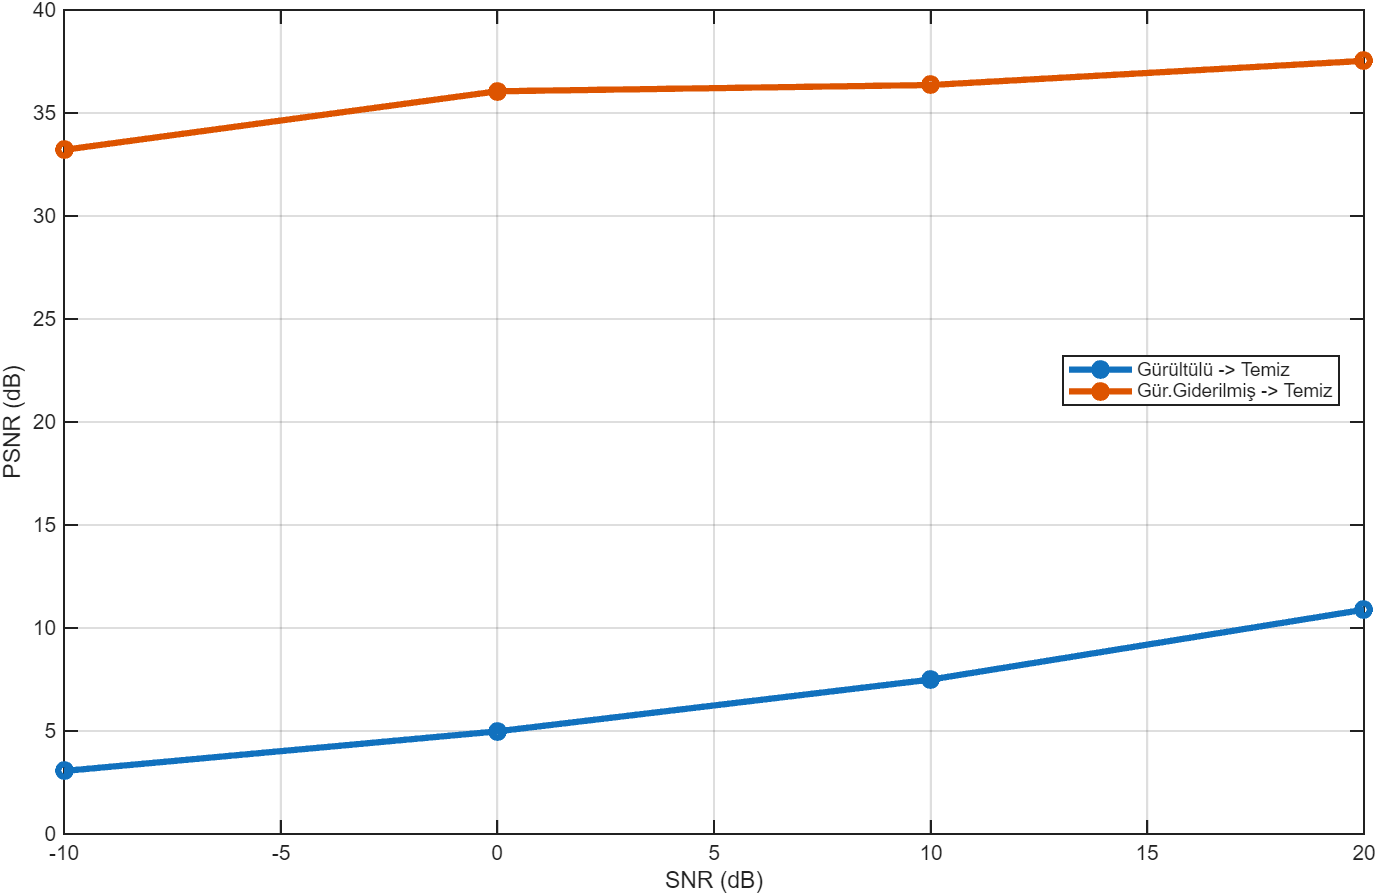
\includegraphics[width=\linewidth]{denoiser_psnr_vs_snr.png}\\
      {\scriptsize PSNR --- SNR ilişkisi}
    \end{column}
    \begin{column}{0.5\textwidth}
      \centering
      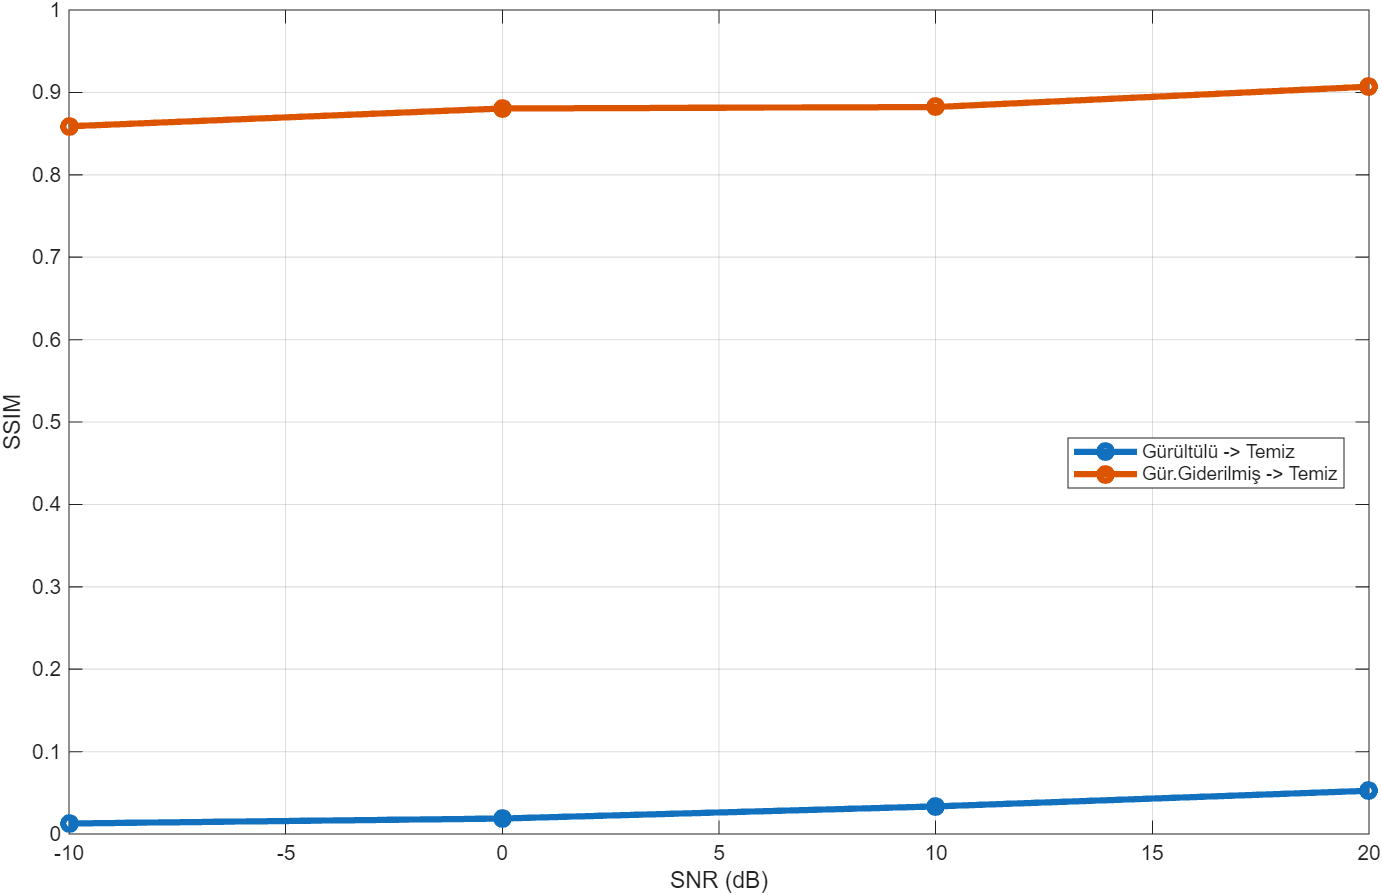
\includegraphics[width=\linewidth]{denoiser_ssim_vs_snr.png}\\
      {\scriptsize SSIM --- SNR ilişkisi}
    \end{column}
  \end{columns}
  \vfill
  \begin{block}{Örnek (tek yama)}\small
    Düşük SNR'lı bir örnekte: PSNR $\;3.5 \rightarrow 22.6$ dB,
    \; SSIM $\;0.04 \rightarrow 0.76$. Denoiser, sinyal yapısını gürültüden
    belirgin biçimde ayırıyor.
  \end{block}
\end{frame}

% =========================================================
\section{Sınıflandırma}
% =========================================================
\begin{frame}{Çok Etiketli Sınıflandırma}
  \begin{columns}[T]
    \begin{column}{0.56\textwidth}
      \begin{itemize}\small
        \item Omurga: ImageNet ön-eğitimli \textbf{GoogLeNet}.
        \item Son katman \textbf{7 çıkışlı sigmoid} (softmax değil)
              $\Rightarrow$ her sınıf bağımsız değerlendirilir.
        \item \textbf{Kayıp fonksiyonu:} ağırlıklı BCE $+$ yumuşak-IoU $+$
              yumuşak-küme terimleri.
        \item Sınıf dengesizliği için \textbf{pozitif/negatif ağırlıklar}.
        \item Her sınıf için \textbf{ayrı karar eşiği} (val setinde optimize).
      \end{itemize}
      \begin{block}{Eğitim}\scriptsize
        Adam, $\text{lr}=3\times10^{-4}$ \;|\; 5 epoch warmup $+$ kosinüs azalma
        \;|\; batch $=64$ \;|\; 60 epoch \;|\; gradyan kırpma $=1.0$ \;|\; veri artırma.
      \end{block}
    \end{column}
    \begin{column}{0.44\textwidth}
      \begin{block}{İki model karşılaştırması}\small
        \begin{itemize}
          \item \textbf{classifier}: gürültülü giriş
          \item \textbf{classifierOnDenoised}: denoiser'dan geçmiş giriş
        \end{itemize}
        Soru: \emph{Gürültü giderme sınıflandırmaya ne kadar katkı sağlıyor?}
      \end{block}
    \end{column}
  \end{columns}
\end{frame}

\begin{frame}{Değerlendirme Metrikleri}
  \begin{itemize}
    \item \textbf{Subset accuracy:} yamanın \emph{tüm} etiketlerinin aynı anda
          doğru olma oranı (en katı ölçüt).
    \item \textbf{Makro-F1:} sınıf başına F1'in ortalaması (nadir sınıflara duyarlı).
    \item \textbf{Sınıf başı F1:} hangi modülasyonun daha kolay/zor ayrıldığını gösterir.
    \item \textbf{Denoiser:} PSNR ve SSIM (temiz referansa göre).
  \end{itemize}
  \vfill
  \begin{center}
    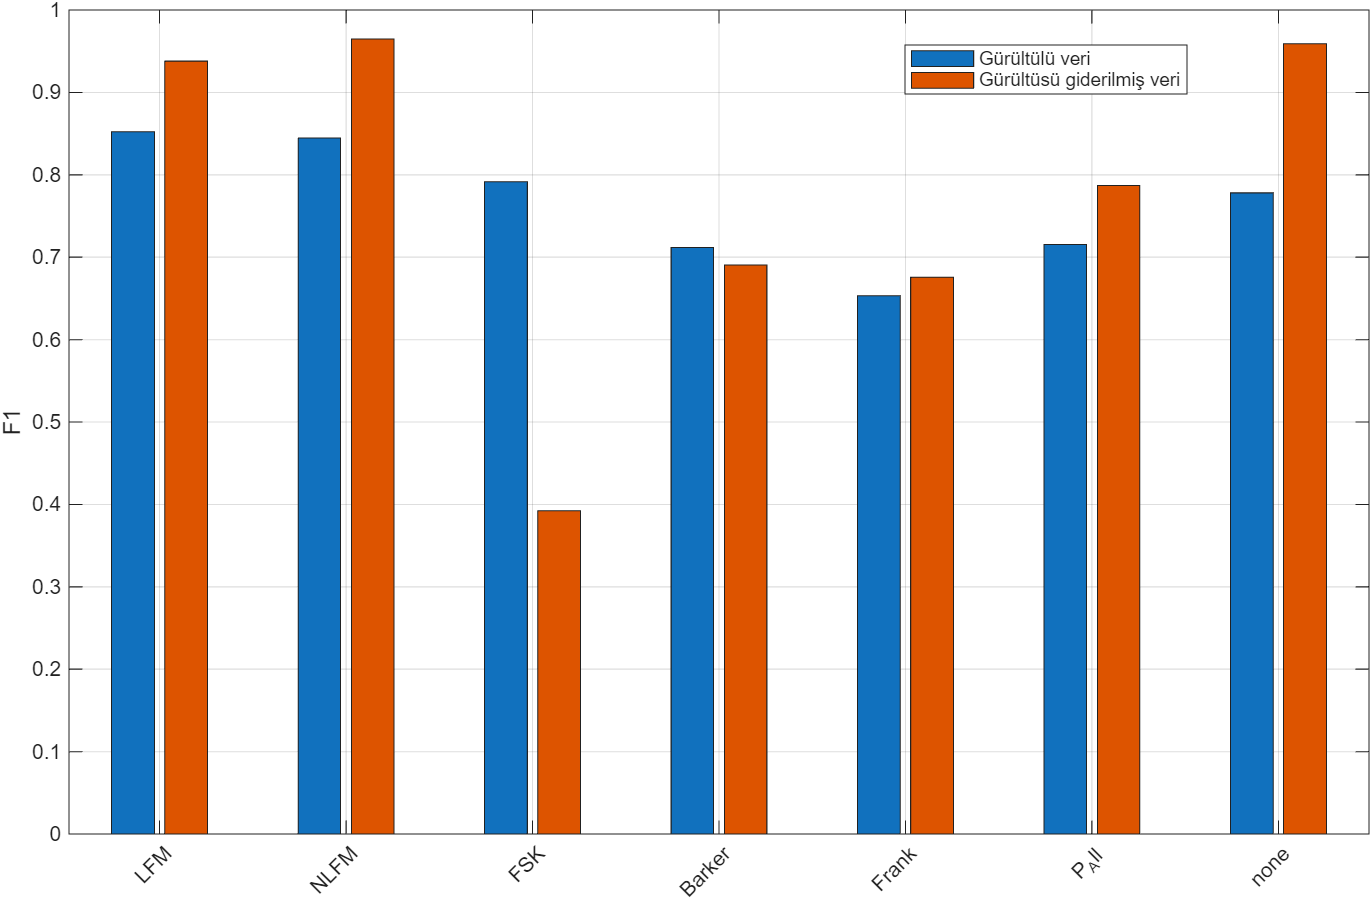
\includegraphics[width=0.62\linewidth]{classifier_perclass_f1.png}\\
    {\scriptsize Sınıf başına F1 --- gürültülü vs. gürültüsü giderilmiş}
  \end{center}
\end{frame}

\begin{frame}{Sınıflandırma Sonuçları}
  \begin{columns}[T]
    \begin{column}{0.5\textwidth}
      \centering
      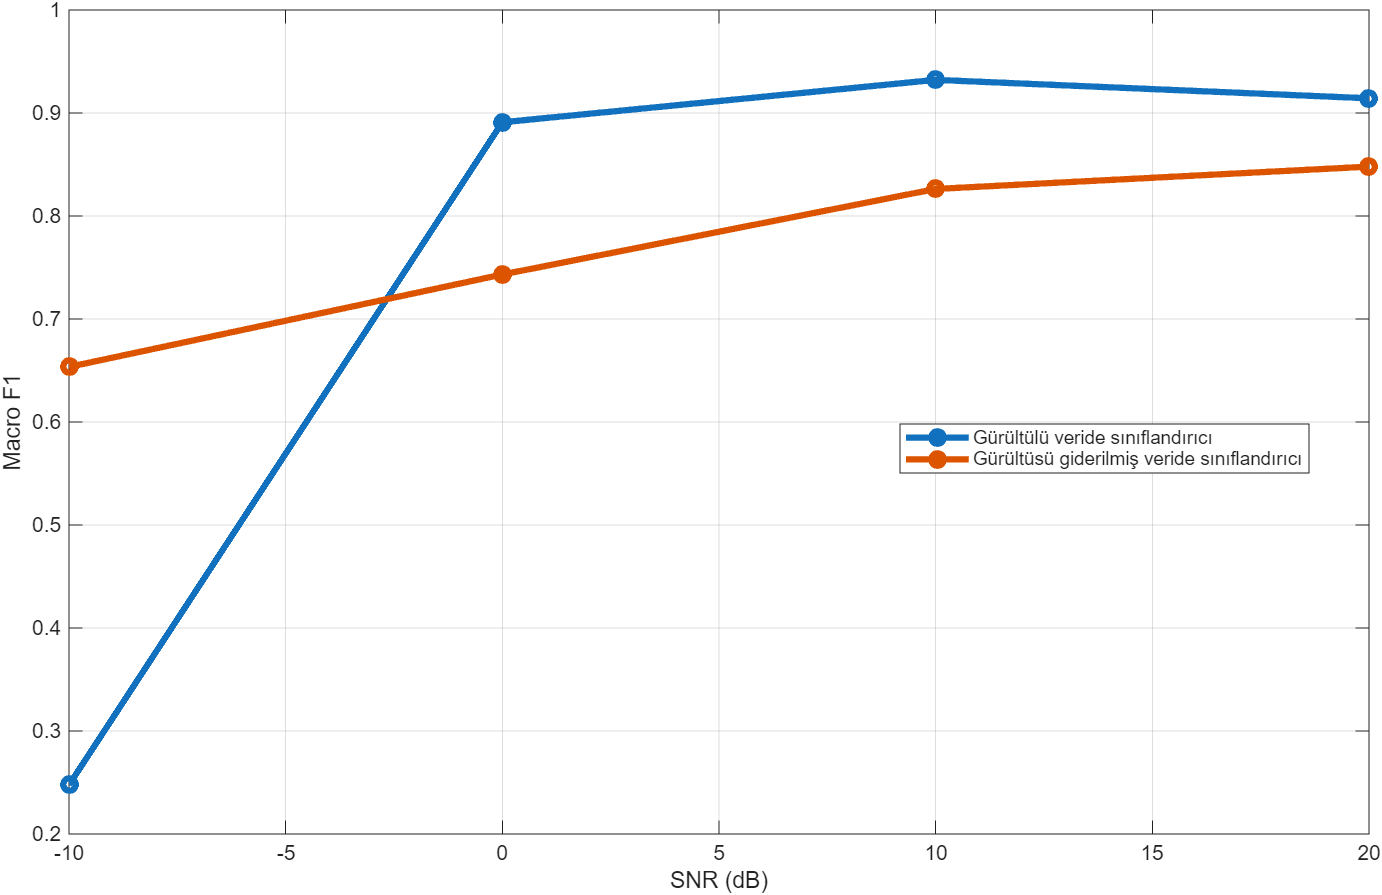
\includegraphics[width=\linewidth]{classifier_macrof1_vs_snr.png}\\
      {\scriptsize Makro-F1 --- SNR}
    \end{column}
    \begin{column}{0.5\textwidth}
      \centering
      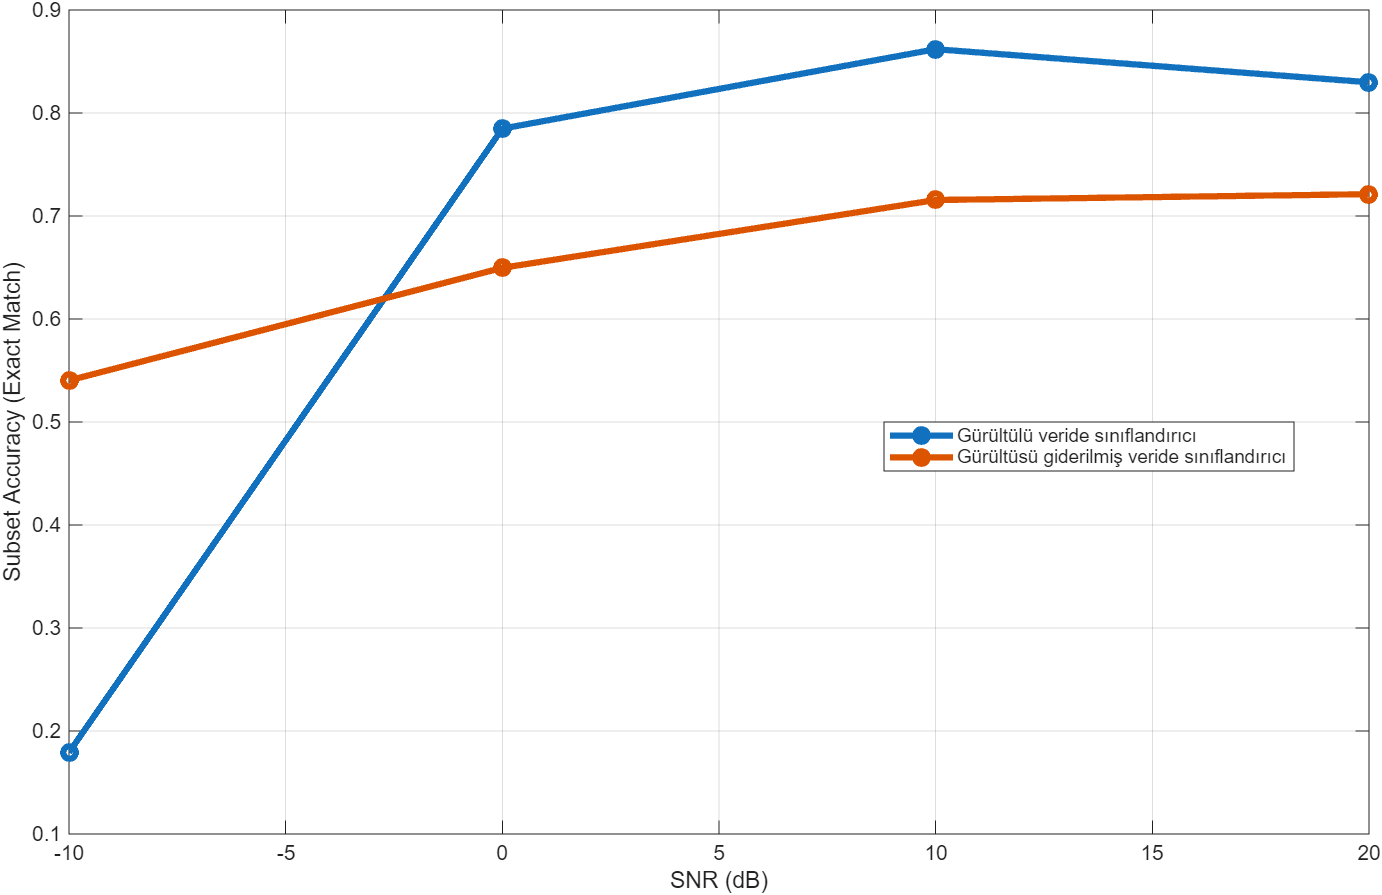
\includegraphics[width=\linewidth]{classifier_subsetacc_vs_snr.png}\\
      {\scriptsize Subset accuracy --- SNR}
    \end{column}
  \end{columns}
  \vfill
  \begin{center}\small
    Gürültü giderme, özellikle \textbf{düşük SNR}'da başarımı yükseltiyor;
    yüksek SNR'da iki model birbirine yaklaşıyor.
  \end{center}
\end{frame}

% =========================================================
\section{Parametre Çıkarımı}
% =========================================================
\begin{frame}{Kenar Tespiti ve RDW Çıkarımı}
  \centering
  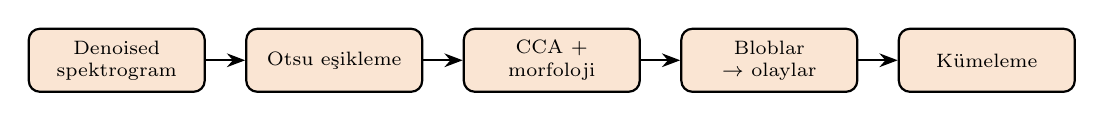
\begin{tikzpicture}[
      node distance=5mm,
      s/.style={draw, rounded corners, fill=cEdge!20, font=\scriptsize,
                minimum height=8mm, text width=2.0cm, align=center},
      >={Stealth[]}, thick]
    \node[s] (a) {Denoised spektrogram};
    \node[s, right=of a] (b) {Otsu eşikleme};
    \node[s, right=of b] (c) {CCA + morfoloji};
    \node[s, right=of c] (d) {Bloblar $\to$ olaylar};
    \node[s, right=of d] (e) {Kümeleme};
    \draw[->](a)--(b);\draw[->](b)--(c);\draw[->](c)--(d);\draw[->](d)--(e);
  \end{tikzpicture}
  \vfill
  \begin{itemize}\small
    \item Olaylar \textbf{PRI, PW, BW, $F_c$} toleranslarıyla kümelenir;
          \textbf{periyodiklik skoru} ile darbe dizileri ayrılır.
    \item Çıktı: olay tablosu, küme etiketi, PRI tahmini ve \textbf{sınır kutuları}
          $\Rightarrow$ \textbf{Radar Tanımlayıcı Kelime (RDW)}.
    \item \texttt{auto\_tune\_threshold\_params}: eşik/son-işlem parametrelerini
          \textbf{yer gerçeğine göre} otomatik ayarlar.
  \end{itemize}
\end{frame}

% =========================================================
\section{Gerçek Zamanlı Uygulanabilirlik}
% =========================================================
\begin{frame}{Gerçek Zamanlı Uygulanabilirlik ve Gecikme}
  \begin{columns}[T]
    \begin{column}{0.52\textwidth}
      \textbf{Ölçülen çıkarım gecikmesi}\\[1pt]
      {\scriptsize ($224\times224$ yama, CPU; GPU'da $5$--$20\times$ daha hızlı)}
      \vspace{1.5mm}
      \renewcommand{\arraystretch}{1.25}
      \begin{tabular}{@{}lr@{}}
        \toprule
        \textbf{İşlem} & \textbf{Süre} \\
        \midrule
        Denoiser                        & $\sim$50 ms \\
        Sınıflandırıcı                  & $\sim$36 ms \\
        Denoiser $+$ Sınıf.\ zinciri     & $\sim$86 ms \\
        Uzun spektrogram ($\approx$19 yama) & $\sim$1.6 s \\
        \bottomrule
      \end{tabular}
    \end{column}
    \begin{column}{0.48\textwidth}
      \textbf{Değerlendirme}
      \begin{itemize}\small
        \item Yama-bazlı ve \textbf{durumsuz} $\Rightarrow$ akışa (pipeline) uygun.
        \item Karar başına gecikme (GPU'da onlarca ms) ESM için kabul edilebilir.
        \item Kesintisiz tam kapsama (her $5$ ms'lik pencere) mevcut haliyle sıkı.
      \end{itemize}
    \end{column}
  \end{columns}
  \vspace{1.5mm}
  \begin{block}{Online'a taşımak için}\small
    GPU $+$ batch çıkarım \;$\bullet$\; örtüşmeyi azalt \;$\bullet$\;
    adaptif denoise (yüksek SNR'da atla) \;$\bullet$\; model hafifletme
    (quantization / pruning) \;$\bullet$\; uçtan uca birleştirme
  \end{block}
\end{frame}

% =========================================================
\section{Sonuç}
% =========================================================
\begin{frame}{Özet ve Gelecek Çalışma}
  \begin{block}{Özet}
    \begin{itemize}\small
      \item Uçtan uca: \textbf{denoise $\rightarrow$ sınıflandır $\rightarrow$
            parametre çıkar}, tek veri setinden beslenen modüler yapı.
      \item Öğren-tabanlı gürültü giderme, düşük SNR'da hem görüntü kalitesini
            (PSNR/SSIM) hem de sınıflandırma başarımını belirgin biçimde artırır.
    \end{itemize}
  \end{block}
  \begin{block}{Gelecek çalışma}
    \begin{itemize}\small
      \item Gerçek (kaydedilmiş) radar verisi üzerinde doğrulama.
      \item Denoiser ve sınıflandırıcının \textbf{uçtan uca ortak eğitimi}.
      \item Spektrogram penceresi ve yan-lob bastırımı için ek iyileştirmeler.
    \end{itemize}
  \end{block}
  \vfill
  \begin{center}\Large Teşekkürler\end{center}
\end{frame}

\end{document}
